
% Experement data + calcs goes here %

\section{Ход работы}

\subsection{Схема установки}

Схема установки представлена на рисунке 2.

\pic{0.8\linewidth}{scheme2.jpg}{Схема установки}

\newpage

\subsection{Динамический метод}

Сняли осциллограммы при максимальном ускоряющем напряжении для трех различных значений
задерживающего напряжения: 4, 6 и 8 В. Измерили на экране расстояние между максимумами
и между минимумами осциллограммы. Результаты измерений занес в таблицу 1. Фотографии
полученных осциллограмм приведены на рисунках 3-5. \\

\shiftedText{0cm}{0.4\linewidth}
{
    \begin{center}
        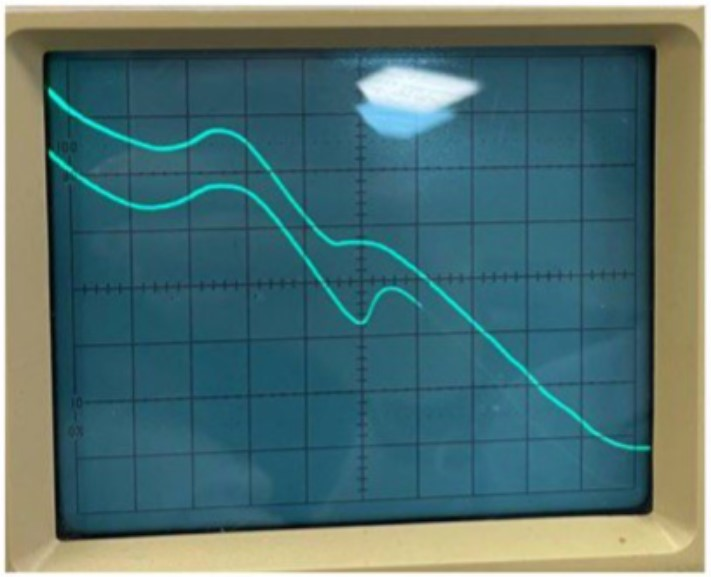
\includegraphics[width = \textwidth]{oscil1.jpg}
        \textit{Рис \arabic{PicsCounter}. ВАХ для $ 4 $ В}
    \end{center}

    \stepcounter{PicsCounter}
} \shiftedText{0cm}{0.4\linewidth}
{
    \begin{center}
        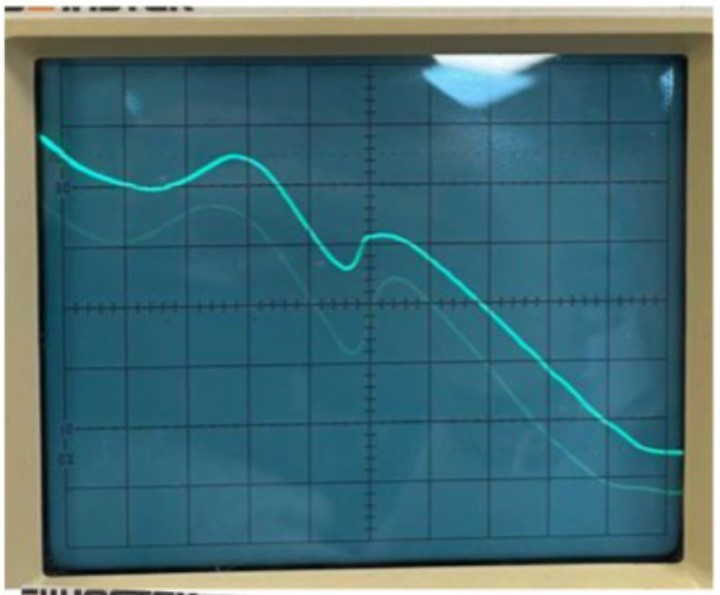
\includegraphics[width = \textwidth]{oscil2.jpg}
        \textit{Рис \arabic{PicsCounter}. ВАХ для $ 6 $ В}
    \end{center}

    \stepcounter{PicsCounter}
}
\pic{0.4\linewidth}{oscil3.jpg}{ВАХ для $ 8 $ В}

\begin{table}[h!]
    \begin{center}
        \tableLable{Данные динамического метода}
        \begin{tabular}{|c|c|c|c|c|}
        \hline
        $ V_2 $, В & $ V_{max_1} $, В & $ V_{max_2} $, В & $ V_{min_1} $, В & $ V_{min_2} $, В  \\ \hline
        4 & -2 & 13 & 2 & 17 \\ \hline
        6 & -2 & 13 & 2 & 20 \\ \hline
        8 & -2 & 13 & 2 & 22 \\ \hline
        \end{tabular}
    \end{center}
\end{table}

Погрешность измерения осциллографа $ \Delta V = 1 $ В.

\newpage

Тогда получил среднее значение энергии первого возбужденного состояния для атома гелия:
\formula{HeliumExcitationEnergyDyn}
{\langle E_{excit_d} \rangle = \left( 16,3 \pm 3,3 \right) \, \texttt{эВ}}

Значение погрешности вычислял по формуле:
\formula{HeliumExcitationEnergyError}
{
    \sigma_{E_{excit}} = 2 \sigma_V + \sigma_{stat} \, , \,
    \sigma_{stat} = \sqrt{\frac{1}{6}\sum{\mid V_i - \langle \Delta E_{excit} \rangle \mid}}
}

\subsection{Статический метод}

Сняли ВАХ для трехэлектродной лампы при трех различных значениях задерживающего напряжения.
Графики представлены на рис. 6. Результаты измерений занес в таблицу 2.

\pic{0.9\linewidth}{graph1.jpg}{ВАХ в статическом методе}

\begin{table}[h!]
    \begin{center}
        \tableLable{Данные статического метода}
        \begin{tabular}{|c|c|c|c|c|}
        \hline
        $ V_2 $, В & $ V_{max_1} $, В & $ V_{max_2} $, В & $ V_{min_1} $, В & $ V_{min_2} $, В  \\ \hline
        4 & 24 & 40 & 25 & 46 \\ \hline
        6 & 24 & 37 & 26 & 47 \\ \hline
        8 & 24 & 38 & 26 & 49 \\ \hline
        \end{tabular}
    \end{center}
\end{table}

Погрешность измерения с графика $ \Delta V = 1 $ В.

Тогда получил среднее значение энергии первого возбужденного состояния для атома гелия:
\formula{HeliumExcitationEnergyStat}
{\langle E_{excit_s} \rangle = \left( 18,0 \pm 3,9 \right) \, \texttt{эВ}}

Значение погрешности вычислял по формуле (\ref{HeliumExcitationEnergyError})

\newpage

\section{Вывод}

В ходе работы были получены наглядные доказательства квантовой теории атомов.

Так же расчетные значения энергии первого возбужденного состояния для атома гелия: \\
\begin{enumerate}
    \item $ \langle E_{excit_s} \rangle = \left( 18,0 \pm 3,9 \right) \, \texttt{эВ} $
    \item $ \langle E_{excit_d} \rangle = \left( 16,3 \pm 3,3 \right) \, \texttt{эВ} $
\end{enumerate}

Cовпадают в пределах погрешности с табличным значением: \\

$ E_{ref} = \left( 19,7 \pm 0,1 \right) \, \texttt{эВ} $
